\cotefile{148}
\scanpage{6}

\noindent
\begin{minipage}[t]{.46\textwidth}
\begin{center}
U N I V E R S I T E\\
DES SCIENCES ET TECHNIQUES\\
DU LANGUEDOC\\
\textasciicircum\textasciicircum\textasciicircum\textasciicircum\textasciicircum\textasciicircum\textasciicircum\textasciicircum\textasciicircum\textasciicircum\textasciicircum\textasciicircum\textasciicircum
\end{center}
\end{minipage}\hfill
\begin{minipage}[t]{.50\textwidth}
\vspace{.9\baselineskip}
Montpellier, le 14 octobre 1983
\end{minipage}

Service de la Scolarité

\begin{tabular}{@{}ll@{}}
Diffusion : & Liste A\\
MA/gs & N° 4375
\end{tabular}

\begin{center}
AVIS DE SOUTENANCE D'UNE THESE DE DOCTORAT DE 3e CYCLE

ECOLOGIE GENERALE ET APPLIQUEE OPTION ECOLOGIE AQUATIQUE

\texttt{========================================================}
\end{center}

\uline{NOM et Prénom du candidat} : MONTI Dominique

\uline{Titre de la thèse} : ``Recherches sur l'optimisation du plan d'échantillonnage employé pour la cartographie des peuplements benthiques. Application à la macrofaune benthique de l'étang de Pierre Blanche (Palavas, Hérault, France).

\uline{Date,-heure et lieu de soutenance prévus} : Le 2 novembre 1983 à 15 heures,\\
Salle de cours n° 9 - Université des Sciences et Techniques du Languedoc

\uline{Nom du Directeur de thèse} : M. AMANIEU

\uline{Désignation du Laboratoire où la thèse est préparée} : Laboratoire d'Hydrobiologie marine - U.S.T.L.

\uline{Analyse de l'ouvrage} : Cette réflexion porte sur le problème du choix du nombre et de l'organisation spatiale des points de prélèvement en écologie. Quel effort doit-on fournir pour un niveau de précision fixé ? Et où doit-on prélever ?

Ce travail est basé sur la réalisation de différents sous-échantillonnages d'une information initiale supposée maximale. Les différents sous-échantillonnages varient par le nombre et l'organisation spatiale des points de prélèvements ; et ils sont tous effectués à partir de la même liste d'objets.

Chaque sous-échantillonnage employé donnera naissance à une carte qui sera par la suite comparée à la carte dite ``de référence'' ; il restera à apprécier au vu de ces résultats si les cartes obtenues diffèrent de la référence, en quelles proportions et de quelle manière.

Les résultats théoriques sont appliqués à l'étude de la macrofaune benthique d'un étang littoral (l'étang de Pierre Blanche à Palavas, France).

\uline{Durée approximative des recherches ayant abouti à la thèse} : 3 ans

\uline{Composition du jury Proposé} : \begin{tabular}[t]{ll}
MM. & AMANIEU M.\\
& BLANC F.\\
& FRONTIER S.\\
& GRANDJOUAN G.\\
& LASSERRE G.
\end{tabular}

\begin{flushright}
P/ le Secrétaire Général,\\
L'Attachée Principale d'Administration\\
Scolaire et Universitaire,

\handwritten{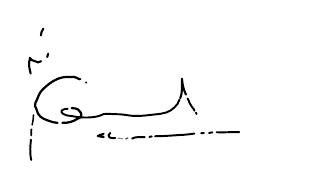
\begin{tikzpicture}[x=0.0013cm,y=-0.0013cm,line cap=round,line join=round]
\draw[line width=0.8pt] (812,700) .. controls (770,691) and (767,669) .. (719,678) .. controls (607,667) and (524,724) .. (445,800) .. controls (403,838) and (398,892) .. (375,927) .. controls (361,945) and (370,973) .. (384,995) .. controls (398,1060) and (437,1085) .. (499,1105) .. controls (538,1119) and (563,1127) .. (590,1127);
\draw[line width=0.8pt] (638,1127) .. controls (697,1130) and (749,1111) .. (780,1090) .. controls (824,1074) and (831,1051) .. (817,1026) .. controls (807,1002) and (787,984) .. (729,982);
\draw[line width=0.7pt] (690,989) .. controls (647,990) and (622,1005) .. (630,1024) .. controls (644,1046) and (686,1058) .. (719,1059) .. controls (758,1061) and (787,1076) .. (835,1074) .. controls (925,1077) and (972,1069) .. (1012,1054) .. controls (1047,1029) and (1093,1041) .. (1154,1042) .. controls (1219,1041) and (1262,1051) .. (1310,1057) .. controls (1403,1066) and (1479,1050) .. (1550,1044) .. controls (1629,1037) and (1690,1023) .. (1732,978) .. controls (1759,958) and (1776,930) .. (1784,900);
\draw[line width=0.75pt] (1792,886) .. controls (1812,837) and (1810,784) .. (1809,694) .. controls (1812,744) and (1824,803) .. (1848,850);
\draw[line width=0.7pt] (1864,888) .. controls (1882,920) and (1887,951) .. (1905,969) .. controls (1923,984) and (1928,1000) .. (1931,1008);
\draw[line width=0.7pt] (1946,1027) -- (1952,1040);
\draw[line width=0.55pt] (355,1050) .. controls (354,1079) and (350,1113) .. (342,1147);
\draw[line width=0.65pt] (334,1191) -- (332,1250);
\draw[line width=0.7pt] (330,1292) .. controls (325,1340) and (316,1414) .. (332,1490);
\draw[line width=0.75pt] (327,644) .. controls (319,607) and (308,570) .. (312,539) .. controls (315,516) and (319,500) .. (320,491) .. controls (324,514) and (346,514) .. (367,522) .. controls (390,535) and (413,544) .. (429,523);
\draw[line width=0.75pt] (427,271) .. controls (429,242) and (438,221) .. (452,205);
\draw[line width=0.75pt] (489,482) -- (499,450);
\fill (870,732) ellipse [x radius=10,y radius=12];
\draw[line width=0.75pt] (1042,1235) .. controls (1020,1242) and (993,1247) .. (984,1256) .. controls (1003,1257) and (1025,1266) .. (1043,1266);
\draw[line width=0.7pt] (1107,1226) .. controls (1087,1238) and (1082,1258) .. (1099,1270) .. controls (1115,1277) and (1141,1280) .. (1156,1275);
\draw[line width=0.45pt,opacity=0.45] (1183,1277) -- (1229,1282);
\draw[line width=0.55pt,opacity=0.65] (1259,1284) -- (1278,1276);
\draw[line width=0.7pt] (1321,1281) .. controls (1350,1263) and (1390,1266) .. (1444,1267);
\draw[line width=0.7pt] (1490,1265) -- (1513,1260);
\draw[line width=0.7pt] (1545,1258) .. controls (1660,1257) and (1735,1248) .. (1827,1244) .. controls (1871,1239) and (1901,1238) .. (1930,1232);
\draw[line width=0.7pt] (1997,1228) -- (2024,1226);
\draw[line width=0.7pt] (2074,1226) -- (2107,1220);
\draw[line width=0.7pt] (2149,1219) .. controls (2220,1224) and (2290,1214) .. (2370,1218);
\node[anchor=west] at (2430,850) {$\unsure{\phantom{A}}$};
\end{tikzpicture}}

A. GENTIL
\end{flushright}

\margin{5}
